\documentclass[tikz,border=10pt]{standalone}
\usepackage{tikz}
\usetikzlibrary{shapes.geometric, arrows, positioning, fit, backgrounds, calc}

\begin{document}

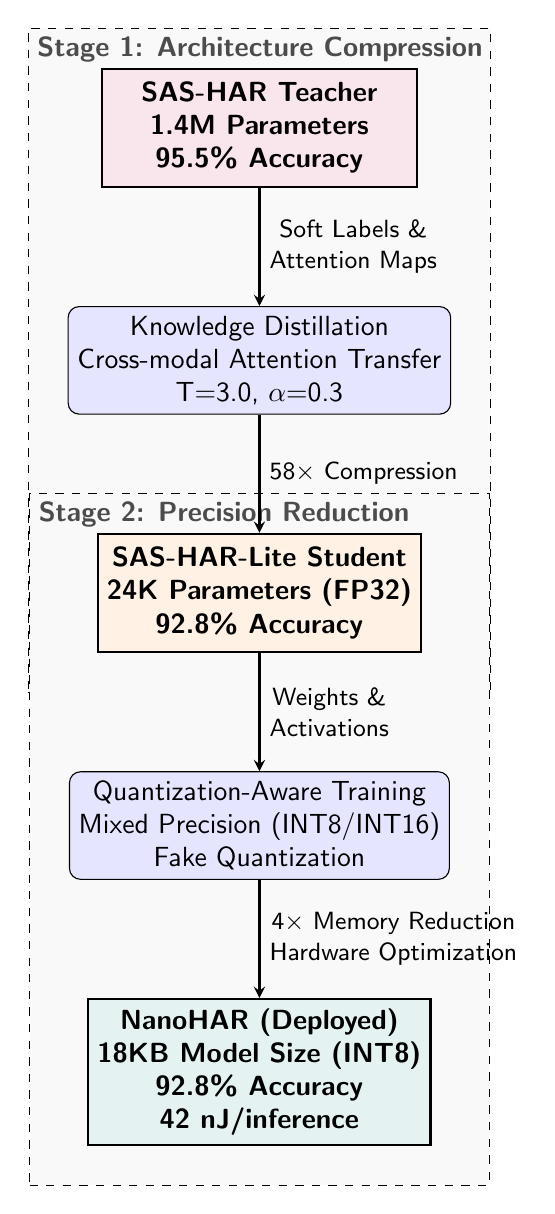
\begin{tikzpicture}[
    node distance=2cm and 2cm,
    box/.style={rectangle, draw, rounded corners, minimum width=3cm, minimum height=1cm, align=center, fill=blue!10, font=\sffamily},
    model/.style={rectangle, draw, thick, minimum width=4cm, minimum height=1.5cm, align=center, fill=green!10, font=\sffamily\bfseries},
    arrow/.style={thick, ->, >=stealth},
    label/.style={font=\sffamily\small, align=center}
]

% Nodes
\node[model, fill=purple!10] (teacher) {SAS-HAR Teacher\\1.4M Parameters\\95.5\% Accuracy};

\node[box, below=1.5cm of teacher] (kd) {Knowledge Distillation\\Cross-modal Attention Transfer\\T=3.0, $\alpha$=0.3};

\node[model, fill=orange!10, below=1.5cm of kd] (student) {SAS-HAR-Lite Student\\24K Parameters (FP32)\\92.8\% Accuracy};

\node[box, below=1.5cm of student] (qat) {Quantization-Aware Training\\Mixed Precision (INT8/INT16)\\Fake Quantization};

\node[model, fill=teal!10, below=1.5cm of qat] (nanohar) {NanoHAR (Deployed)\\18KB Model Size (INT8)\\92.8\% Accuracy\\42 nJ/inference};

% Arrows
\draw[arrow] (teacher) -- (kd) node[midway, right, label] {Soft Labels \&\\Attention Maps};
\draw[arrow] (kd) -- (student) node[midway, right, label] {58$\times$ Compression};
\draw[arrow] (student) -- (qat) node[midway, right, label] {Weights \&\\Activations};
\draw[arrow] (qat) -- (nanohar) node[midway, right, label] {4$\times$ Memory Reduction\\Hardware Optimization};

% Background boxes for stages
\begin{scope}[on background layer]
    \node[draw, dashed, inner sep=0.5cm, fill=gray!5, fit=(teacher) (kd) (student)] (stage1) {};
    \node[anchor=north west, font=\sffamily\bfseries, text=black!70] at (stage1.north west) {Stage 1: Architecture Compression};
    
    \node[draw, dashed, inner sep=0.5cm, fill=gray!5, fit=(student) (qat) (nanohar)] (stage2) {};
    \node[anchor=north west, font=\sffamily\bfseries, text=black!70] at (stage2.north west) {Stage 2: Precision Reduction};
\end{scope}

\end{tikzpicture}

\end{document}